\chapter{Analyse des besoins}

\section{Objectifs et motivations}
La génération automatique de terrains virtuels est un problème sur lequel
planchent souvent les graphistes et les games designers, car pouvoir créer
 un monde virtuel persistant est une brique de base à de nombreuses
applications. Mais, même si le sujet a été maintes fois traité, il reste un
problème difficile non seulement techniquement à cause de la masse de calculs
 que cela représente mais aussi parce que le rendu final du paysage doit
paraître un tant soit peu réaliste aux yeux des utilisateurs.\\

Le but de ce projet est de créer une bibliothèque permettant la création de
terrains virtuels à partir de méthodes fractales ou de bruits. L'utilisateur de la bibliothèque
pourra réaliser des cartes carrées ou sphériques et disposera d'un choix
conséquent d'algorithmes de génération.
La bibliothèque permettra aussi la visualisation des terrains avec différents
niveaux de détails. \\

\section{Interopérabilité entre la bibliothèque et certains visualisateurs existants}
Il existe de nombreux visualisateurs capables de créer un terrain à partir de cartes d'élévations et / ou de modèles externes.
Ainsi il sera intéressant de combiner le réalisme des cartes d'élévations et des modèles générés avec le rendu proposé par ces visualisateurs. Ceux choisis sont TerraGen3 (référence pour le travail de terrains) et Blender3D (open-source et très efficace pour le travail de modèles). 
Les terrains pourront également être importés. Un visualisateur personnel pourra aussi être amené au projet mais la conception de ce dernier n'est pas une priorité.

\section{Scénario d'exécution}
La figure ci-après présente un scénario d'utilisation de notre
bibliothèque.
L'utilisateur spécifie les paramètres qu'il souhaite aux différentes composantes de
celle-ci. Effectivement, il aura accès aux principales structures (carte d'élévation,
grille, etc).
Les modules de la bibliothèque pourront être utilisés de façon indépendante même s'il
est évident que certains modules doivent être utilisés avant d'autres (e.g : création du terrain avant visualisation).


\begin{figure}[!ht]
    \begin{center}
        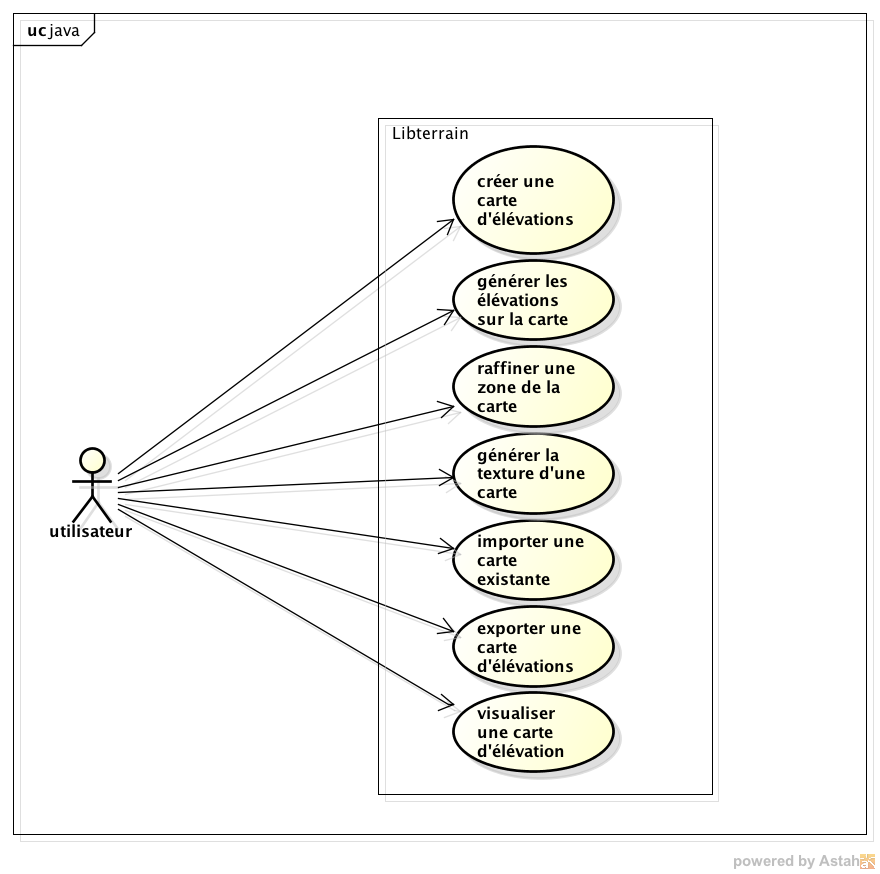
\includegraphics[width=15cm]{resources/use-case.png}
        \label{fig:use_case}
        \caption{Scénario d'exécution}
    \end{center}
\end{figure}

\section{Besoins fonctionnels}

\subsection{Besoins prioritaires}

Ces besoins sont ceux que nous nous engageons à implémenter.

\subsubsection{Structures de données}
La bibliothèque devra proposer deux types de cartes d'élévations :\\
\textbf{sphériques} et \textbf{carrées}.

\subsubsection{Algorithmes de générations de terrains}
Pour permettre la génération d'un terrain, les méthodes suivantes devront pouvoir
 être appliquées sur les cartes d'élévation (les méthodes suivies de la mention [prioritaire] sont celles qui doivent \^etre implémentées en priorité) :\\

\noindent méthodes des fractales :
\begin{itemize}
\item diamond-square ; [prioritaire]
\item midpoint displacement ; [prioritaire]
\item fractional brownian motion ;
\item multi-fractal midpoint displacement.
\end{itemize}
méthodes des bruits :
\begin{itemize}
\item simple noise ;
\item cell noise ;
\item Perlin noise ; [prioritaire]
\item value noise.
\end{itemize}
raffinement par modèles :
\begin{itemize}
\item erosion model.
\end{itemize}

\subsubsection{Raffinement d'un terrain}
S'il souhaite raffiner une zone précise, l'utilisateur pourra la sélectionner (en passant ses coordonnées en paramètres) afin d'appliquer une des méthodes de raffinement (de son choix) sur cette seule zone.

\subsubsection {Génération d'une grille}
Pour les cartes carrées et sphériques, il sera possible de choisir une grille carrée, triangulaire ou hexagonale.

\subsubsection{Importation / exportation}
Les cartes d'élévations pourront être importées et exportées sous forme
d'images (.png, .jpeg) afin d'être lisible par d'autres logiciels
tels que Terragen 3 ou Blender 3D. \newline
Les modèles sont exportés sous format .obj pour être lisible par Blender3D.
Une méthode sera donc conçue pour lire les fichiers importés et une autre pour les concevoir dans le cas d'un export. 

\subsection{Besoins non prioritaires}

\subsubsection{Génération de texture}
Il devra être possible de donner une couleur différente à chaque point de la carte en
fonction de son élévation.

\subsubsection{Implémentation d'un visualisateur 3D}
Génération d'une simple représentation de la carte par rapport à la
carte d'élévation d'origine et du modèle construit par la bibliothèque.

Implémentation d'un zoom pour pouvoir visualiser la carte avec différents niveaux
de détail.


\section{Besoins non fonctionnels}

\subsection{Comportement}

\subsubsection{Performances}
La génération de terrains n'étant pas faite en temps réel, aucune exigence
concernant la vitesse de calcul n'est spécifiée : la qualité du rendu prime sur
le temps d'exécution. Le temps de génération de nos terrains pourra donc \^etre conséquent (de quelques secondes à quelques minutes).\\

Il n'y a pas d'interactivité entre l'utilisateur et le programme pendant l'exécution de ce dernier (le programme peut donc s'exécuter en tâche de fond).\\

\subsubsection{Facilité d'utilisation}
La bibliothèque devra \^etre facile à prendre en main pour l'utilisateur (qui sera un développeur) et devra proposer un maximum d'algorithmes de génération de terrains (parmis ceux qui sont décrits dans les besoins fonctionnels).\\

Il s'agit de développer une bibliothèque et non un logiciel. L'utilisateur
de notre projet est donc un développeur. En conséquence il n'est pas demandé
d'implémenter d'interface graphique pour l'utilisation de la bibliothèque elle-m\^eme, l'utilisateur final pourra, s'il le souhaite, en créer une en s'appuyant sur les différents services proposés par notre bibliothèque.\\

\paragraph{Contraintes :}
Une documentation devra être livrée avec la bibliothèque.

\paragraph{Validation :}
Plusieurs programmes d'exemples illustrant l'utilisation de notre bibliothèque seront livrés.

\paragraph{Portabilité :}
La bibliothèque sera développée pour les plateformes Linux/x86 et devra utiliser
GNU Autotools comme système de construction.

\subsubsection{Contraintes}
Toute utilisation de bibliothèque devra \^etre justifiée afin d'éviter la prolifération des dépendances. La bibliothèque boost ne devra \^etre utilisée qu'en cas d'absolue nécessité.

\subsubsection{Persistance des données de la génération procédurale}
Les exécutions avec les mêmes paramètres (méthodes, graine aléatoire, etc)
doivent fournir le même résultat.

\paragraph{Validation :}
Pour N exécution d'une méthode avec des paramètres identiques, comparer les cartes d'élévations obtenues (sommet par sommet) en vérifiant que les sommets aient les mêmes élévations. 

\subsection{Besoins organisationnels}

\subsubsection{Langage}
L'implémentation sera faite en C++.

\subsubsection{Style de codage}
Le projet devra respecter le style de codage de linux :\\
\url{https://www.kernel.org/doc/Documentation/CodingStyle}\\
\emph{(Dernière visite : 10/02/2014)}
%\subsection{Gestion du temps}
%% TODO diagramme Gant


\subsection{Autres besoins}

\subsubsection{Contraintes légales}
Le projet sera distribué sous Licence Publique Générale Limitée GNU (GNU LGPL).

Nous avons choisi cette licence car c'est une licence de logiciel libre mais
moins contraignante que la GPL. En effet elle autorise à lier un programme
développé sous cette licence à du code non (L)GPL. Il sera donc possible d'utiliser notre bibliothèque dans un programme publié sous une autre licence sans révoquer celle-ci.

\subsubsection{Contraintes d'interopérabilité}
Notre bibliothèque hérite de certains modules provenant de LibNoise. 
Ainsi, il faut respecter les interfaces des modules de Libnoise (typage, etc).
Les cartes d'élévation produites par notre bibliothèque devront être lisible par les visualisateurs
 suivants : TerraGen 3 et Blender 3D.\\
\textbf{Terragen 3} utilise des fichiers au format .TER et les modélise sous forme de terrains.\\
Pour \textbf{Blender 3D}, les traitements en amont sont plus simples car ce logiciel charge
une carte d'élévation (image en niveaux de gris) et sous forme de modèle (fichiers
.obj).
Les configurations se font ensuite depuis Blender 3D.

